%% BEGIN PREAMBLE %%%%%%%%%%%%%%%%%%%%%%%%%%%%%%%%%%%%%%%%%%%%%%%%%%%%%%%%%%%%%%

% LaTeX documents have a preamble. It's where you set up all styles, commands,
% and packages. (As you can see, percent signs (%) are used to comment out
% sections in LaTeX documents.)

% This is one default document class; this should go at the top of the file
\documentclass[12pt]{article}


%% PACKAGES

% Packages are add-ons that allow you to modify the default structure of
% a LaTeX document. You call them up here. Most packages are automatically
% downloaded with the TeX distribution you have. Some have to be downloaded
% separately, but it's not a big deal. I don't really know why LaTeX doesn't
% just have these as options without calling up packages. Maybe just the
% history of the system or to save space. Below are just some examples.
% There are tons of packages.

\usepackage{times} % Times font
\usepackage{titlesec} % Titles can be formatted
\usepackage{tabularx} % This allows for more fluid tables (see below)
\usepackage{booktabs} % This helps make neater tables (see below)
\usepackage[margin=1in, paperwidth=8.5in, paperheight=11in]{geometry} % Margins
\usepackage{caption} % Captions more adjustable
\usepackage{fancyhdr} % Lets you make nice headers and footers
\usepackage{longtable} % Allows for table that floats across pages
\usepackage{rotating} % Allows for sideways tables
\usepackage{setspace} % Can set the spacing of discrete sections of the document
\usepackage{graphicx} % More control over figures (images)
\usepackage{apacite} % Sets up APA style in-text citation system for document
\usepackage{url} % Urls in APA bibliography do not change to monospace font
\usepackage{enumerate} % Gives you more control over lists
\usepackage{amsmath} % Much more powerful equation editor

%% COMMANDS

% LaTeX allows you to create your own commands. This is really nice if there
% is something you do a lot that normally requires a long or just annoying
% command structure. Below, I've just created commands that are shortened
% versions of longer ones.

\newcommand{\RR}{\raggedright\arraybackslash} % Allows left align in tables
\newcommand{\RL}{\raggedleft\arraybackslash} % Allows right align in tables
\newcommand{\indentitem}{\setlength\itemindent{1.5em}} % Manually add indent

%% STYLES

% Using the packages loaded above, I'm able to set up some general page styles.
\pagestyle{fancy} % Calls up the fancyhdr package above
% Right header with my name and the automatic page number
\fancyhead[R]{\scshape Benjamin Skinner $\vert$ \thepage}
% Left header with document title
\fancyhead[L]{\scshape \LaTeX{} Example Document}
% Nothing in the footer (i.e. remove automatic page numbers in footer)
\fancyfoot{}
\renewcommand{\headrulewidth}{0.4pt} % Sets the thickness of the header line

% Change font of section/subsection headers b/c I want to do so
\titleformat*{\section}{\Large\scshape} % To small caps
\titleformat*{\subsection}{\scshape} % To small caps, smaller font

% Setting up title page
\title{\huge\scshape \LaTeX{} \\ {\Large The Clear Plastic Binder of Social Science Research}}\label{doc:title}
\date{{\scshape Last updated} \\ \scshape{\today}}
\author{\scshape{\Large Benjamin Skinner}}

%% END PREAMBLE	%%%%%%%%%%%%%%%%%%%%%%%%%%%%%%%%%%%%%%%%%%%%%%%%%%%%%%%%%%%%%%%%
%% BEGIN DOCUMENT %%%%%%%%%%%%%%%%%%%%%%%%%%%%%%%%%%%%%%%%%%%%%%%%%%%%%%%%%%%%%%

\begin{document}
\maketitle % Takes the title commands in the preamble and places it in document
\tableofcontents
\thispagestyle{empty} % Removes header/footer from front page
\newpage

\section*{License} % License preamble section
% NB: * (an asterisk) turns off numbering; remove to turn it back on
{\parindent0pt % disables indentation for all the text until closing }

Document produced by: \\

Benjamin Skinner \\
PhD Student, Leadership and Policy Studies \\
Peabody College, Vanderbilt University \\
\url{https://my.vanderbilt.edu/benjaminskinner/} \\

Copyright (C) 2012 Benjamin Skinner. All rights reserved. \\

This document is free: you can redistribute it and/or modify
it under the terms of the GNU General Public License as published by
the Free Software Foundation, either version 3 of the License, or
(at your option) any later version. \\

This document is distributed in the hope that it will be useful,
but WITHOUT ANY WARRANTY; without even the implied warranty of
MERCHANTABILITY or FITNESS FOR A PARTICULAR PURPOSE.  See the
GNU General Public License for more details. \\

You should have received a copy of the GNU General Public License
along with this document.  If not, see \url{http://www.gnu.org/licenses/}.
}

\cleardoublepage % Making new page (not necessary when using APA document class)

\section*{Welcome to \LaTeX{}} % Start section

\LaTeX{} is a document preparation system that is based on a WYSIWYM
model (What you see is what you {\itshape mean}) rather than a WYSIWYG
model (what you see is what you {\itshape get}) like that used by MSWord. 
Though some have called \LaTeX{} a ``solution without a problem"
\cite{philosophicus1927agenda}, its ability to create long and complex 
documents is unparalleled. \LaTeX{} uses its engine to transform .tex files---
which are really just specially coded .txt files---into PDF files that,
regardless of content, look highly professional. In other words,
\LaTeX{} is the clear plastic binder of social science research 
({\itshape c.f.} ``Bats aren't bugs'' strips in \cite{watterson1992indesp}).

\begin{figure*}[h!]
\caption{A+ Work Flow}
\noindent 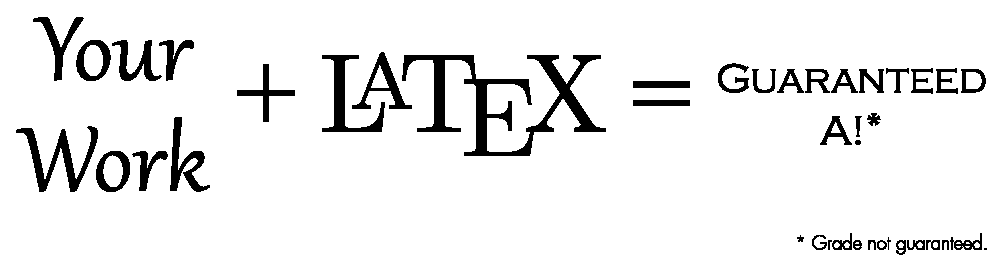
\includegraphics[width=\linewidth]{aplus.eps}
\end{figure*}

To use this document as guide for \LaTeX{}, you will need to refer to
both  the finished PDF file and the .tex file that created it. This means, 
of course, that you will need to have installed a TeX engine on your computer 
(See accompanying README file or just Google it). I have also included the 
.tex code in appendix of this document. Many other (and better) \LaTeX{} guides exist. 
A list of them can be found at http://latex-project.org/guides/.

% NB: LaTeX automatically creates hyperlinks in the digital document
% when http:// is used.

\section{Citations}

When citing, there are a number of different cite commands that allow
for  different sentence structures. \cite{strongrule2012wizards},
\citeA{strongrule2012wizards}, \citeauthor{strongrule2012wizards}, and
\citeyear{strongrule2012wizards} were all created using a different versions of
the {\tt \textbackslash{cite}} command (for above, specifically:
{\tt \textbackslash{cite}}, {\tt \textbackslash{citeA}},{\tt
  \textbackslash{citeauthor}}, and {\tt \textbackslash{citeyear}}). Multiple 
citations can be created by simply including two or more cite keys in the cite
 command separated by a comma: 
\cite{philosophicus1927agenda, strongrule2012wizards}.

% NB: Because certain LaTeX symbols have special meaning in the code
% (& % $ # _ { } ~ ^ \), you have to ``escape" them if you want to
% print them in the text. In cases like those found in the preceding
% paragraph, use the command as shown in the final PDF.

For citations to work, you need an associated .bib file. This is the file 
that holds all the bibliographic information that your sources contain. Many 
PDF managers such as Mendeley will create .bib files for the various working 
folders/libraries you use. Most research databases and Google Scholar will also 
let you export citations in BibTeX format. For citations to populate throughout 
the document properly, your .bib file has to be in the same directory/folder as 
the .tex document or the \LaTeX{} editor you use has to know where to find the 
.bib file (i.e., hard links in the .tex document).

\section{Lists}

You can create a few different types of lists in \LaTeX{}. Three
examples are: enumerate, itemize, description.

\subsection{Enumerate}
\begin{enumerate}[I.] % With the enumerate package, we can change the marker
\item Make a point
\begin{enumerate} % To start a subgroup, just nest another enumerate area
\item Subpoint
\item Subpoint
\end{enumerate}
\item Make another point
\end{enumerate}

\subsection{Itemize}
\begin{itemize}
\item Just
\item some
\item unordered
\item ideas
\end{itemize}

\subsection{Description}
\begin{description}
\item[Put brackets] around the items you want bolded. With enough
  text, you can see that the paragraph is set up with a hanging indent.
\item[Description] is good for defining terms.
\end{description}

\section{Equations}

One of the strengths of \LaTeX{} is its ability to create very nice
equations. As is the case for the entire system, learning the various
equation codes is a pain at first, but worth it in the end.

You can produce inline equations by surrounding the
equation with {\tt \$$\ldots$\$}. An inline equation becomes a bit
squished like so, $\lim_{N \rightarrow \infty} \Pr(\vert \Theta_{N} -
\Theta \vert < \epsilon) = 1$, but inline is good if you only have one
equation within a large body of text. To create full equations that
are numbered, use the \texttt{\textbackslash{begin\{equation\}}} command.

% Begin equation
\begin{equation}
\lim_{N \rightarrow \infty} \Pr(\vert \Theta_{N} - \Theta \vert < \epsilon) = 1
\end{equation}
% End equation

To create an equation without numbering, simply add an asterisk to the
prior command (make sure you have the {\itshape amsmath} package in the
preamble): \texttt{\textbackslash{begin\{equation*\}}}. (Note that
adding an asterisk is the general method for suppressing numbering in
all \LaTeX{} commands that normally add them.) This example equation only 
scratches the surface. There are many more types of equations that \LaTeX{} 
can create. Having a handy symbol guide and a little patience is recommended.


\section{Tables}

\subsection{Everyday Tables}
Tables in \LaTeX{} are the jam. Table \ref{tab:easy} is an easy
one. Notice how Table \ref{tab:easy} is small and without much
text. Had we used more text, \LaTeX{} would have kept it all on one
line and pushed the table outside of the page margins. There are two
ways to have the text wrap and/or set the table to the dimension you
want. The first way is to use the {\itshape tabularx} package. With
{\itshape tabularx} \LaTeX{} can adjust the table to fit whatever
dimensions you set. Table \ref{tab:medium} is an example. If you are a
control freak and absolutely need your table to be a certain size, you
can also set your columns to be specific widths as in Table \ref{tab:mediumer}.

% Easy Table
% h = here
% ! = really
% [!h] = really try to place the thing right here
\begin{table}[!h]
\centering % table align center; otherwise it follows document style
\caption{Easy Table}\label{tab:easy}
% The ``l c r" says that I want three columns that are left aligned,
% center aligned, and  right aligned, respectively. Make sure the
% number of  columns here matches the number you need.
\begin{tabular}{l c r}
\hline % creates a horizontal line
1 & 2 & 3 \\ % Use & to separate columns and \\ to end a line.
\hline
\\ % This gives some space between rows
A & B & C \\
\\
a & b & c \\
\\
$\alpha$ & $\beta$ & $\gamma$ \\
\\
\hline
\end{tabular}
\end{table}

% Medium Table (tabularx)
\begin{table}[!h]
\centering
\caption{Medium Table}\label{tab:medium}
% The X tells LaTeX to set the column width as it sees best; with
% tabularx, you also need to set an overall width in brackets before
% the column brackets. Here, I've told it to be as wide as the length
% a line (i.e. the writable area within the margins).
\begin{tabularx}{\linewidth}{X X X}
\hline
1 & 2 & 3\\
\hline
\\
A & B & C \\
\\
a & b & c \\
\\
$\alpha$ & $\beta$ & $\gamma$ \\
\\
\hline
\end{tabularx}
\end{table}

% Mediumer Table (fixed width column)
\begin{table}[!h]
\centering
\caption{Extra Medium Table}\label{tab:mediumer}
 % The p{} tells the column how wide to be; the >{} before it tells it
 % how to align. You can see that I use some of my homemade commands
 % from above. \RR is much quicker to type than \raggedright\arraybackslash.
\begin{tabular}{>{\RR}p{1in} >{\centering}p{2in} >{\RL}p{1in}}
\hline
1 & 2 & 3\\
\hline
\\
A & B & C \\
\\
a & b & c \\
\\
$\alpha$ & $\beta$ & $\gamma$ \\
\\
\hline
\end{tabular}
\end{table}

\subsection{Cleaner Tables}
Using \texttt{\textbackslash{}hline} when creating tables is a pain,
especially if you want lines that only cover part of the
table. Furthermore, you end up with squished tables. The
{\itshape booktabs} package makes this process easier. See Table
\ref{tab:bettertable} for an example of a slightly more complex, but
more professional-looking table.

% Better Table
\begin{table}[!h]
\centering
\caption{Better Table}\label{tab:bettertable}
\begin{tabular}{>{\RR}p{2in} c c c c}
\toprule
& \multicolumn{2}{l}{Group 1} & \multicolumn{2}{l}{Group 2} \\
\cmidrule(r){2-3}
\cmidrule(r){4-5}
1 & 2 & 3 & 4 & 5\\
\midrule
\\ % This gives some space between rows
A & B & C & D & E\\
\\
a & b & c & d & e\\
\\
$\alpha$ & $\beta$ & $\gamma$ & $\delta$ & $\epsilon$ \\
\\
\bottomrule
\end{tabular}
\end{table}

\subsection{Long Tables}
Sometimes you have a table that is too long and must be spread over
multiple pages. Since the whole point of \LaTeX{} is that it
automatically sets up your document, you need a table that will flow
and break with the page as necessary. The {\itshape longtable} package
allows you to do this. I'm not going to lie, it's a pain to set
up. See Table \ref{tab:long}.

% Long Table
\begin{longtable}{>{\RR}p{2in}>{\centering}p{2in}>{\RL}p{2in}}
\label{tab:long} \\
\caption{Long Table} \\
\toprule % Begin first header
Letter & Number & Greek \\
\midrule
\endfirsthead % End of first header
\multicolumn{2}{l}{\emph{... table \thetable{} continued}} \\ % pb header
\toprule % Repeat header for use after page break (should be the same)
Letter & Number & Greek \\
\midrule
\endhead % all headers finished
\bottomrule % putting in footer before content (way this table works)
\multicolumn{2}{r}{\emph{Continued on next page...}}\\ % pb footer
\endfoot % end of footer
\endlastfoot % since the footer won't change, we can just finish all footers
\\
A & 1 & $\alpha$ \\
\\
B & 2 & $\beta$ \\
\\
C & 3 & $\gamma$ \\
\\
D & 4 & $\delta$ \\
\\
E & 5 & $\epsilon$ \\
\\
F & 6 & $\zeta$ \\
\\
G & 7 & $\eta$ \\
\\
H & 8 & $\theta$ \\
\\
I & 9 & $\iota$ \\
\\
J & 10 & $\kappa$ \\
\\
K & 11 & $\lambda$ \\
\\
L & 12 & $\mu$ \\
\\
M & 13 & $\nu$ \\
\\
N & 14 & $\xi$ \\
\\
O & 15 & $\pi$ \\
\\
P & 16 & $\rho$ \\
\\
Q & 17 & $\sigma$ \\
\\
R & 18 & $\tau$ \\
\\
S & 19 & $\upsilon$ \\
\\
T & 20 & $\phi$ \\
\\
U & 21 & $\chi$ \\
\\
V & 22 & $\psi$ \\
\\
W & 23 & $\omega$ \\
\\
X & 24 &  \\
\\
Y & 25 &  \\
\\
Z & 26 &  \\
\bottomrule
\end{longtable}

\subsection{Tables with External Data}
As you can see from the accompanying .tex file, I've created all the
preceding tables by  hand. While this works for one-off tables with
data that don't change, you want to create tables that will change
automatically if the data coming from a statistical package such as R or
Stata change. The good news is that all you need to do to use an
external table is link to it with the \texttt{\textbackslash{}input}
command in the body of the table. Table \ref{tab:linkeddata} is an
example. Though it looks just like Table \ref{tab:bettertable} in the
formatted PDF, see the .tex file for the difference.

(Of course, I just saved the same data I created before in another
.tex file; to produce the .tex data file automatically with your
favorite statistical software is another matter. My suggestion is to
have the stats software export the data in a .tex format with the
least amount of column, row, and header information possible and use
\LaTeX{} to recreate it: it will look better that way IMNSHO. The
{\itshape estout} package in Stata, with its suite of commands, would be
one way to do this. The {\itshape texreg} library works in R.)

% Better Table (with external file)
\begin{table}[!h]
\centering
\caption{Better Table (with External Data File)}\label{tab:linkeddata}
\begin{tabular}{>{\RR}p{2in} l l l l}
\toprule
& \multicolumn{2}{l}{Group 1} & \multicolumn{2}{l}{Group 2} \\
\cmidrule(r){2-3}
\cmidrule(r){4-5}
1 & 2 & 3 & 4 & 5\\
\midrule
\\ % This gives some space between rows
A & B & C & D & E\\
\\ 
a & b & c & d & e\\
\\
$\alpha$ & $\beta$ & $\gamma$ & $\delta$ & $\epsilon$ \\
\\
\bottomrule
\end{tabular}
\end{table}

\subsection{Sideways Tables}
Other times you need a wide table that is longer than the width of the
page in landscape view. Make sure you have the rotating package called
in the header of the document and simply use the
\texttt{\textbackslash{}sidewaystable} to rotate it. See Table
\ref{tab:sideways} on page \pageref{tab:sideways}.

% Better Table
\begin{sidewaystable} % Use sidewaystable command to rotate table
\centering
\caption{Sideways Table}\label{tab:sideways}
\begin{tabular}{>{\RR}p{3.5in}>{\RR}p{1in}>{\RR}p{1in}>{\RR}p{1in}>{\RR}p{1in}}
\toprule
& \multicolumn{2}{l}{Group 1} & \multicolumn{2}{l}{Group 2} \\
\cmidrule(r){2-3}
\cmidrule(r){4-5}
1 & 2 & 3 & 4 & 5\\
\midrule
\\ % This gives some space between rows
A & B & C & D & E\\
\\
a & b & c & d & e\\
\\
$\alpha$ & $\beta$ & $\gamma$ & $\delta$ & $\epsilon$ \\
\\
\bottomrule
\end{tabular}
\end{sidewaystable}

% Move this part to a new page; sometimes makes things a little
% cleaner, but use sparingly and only at the end...don't fight LaTeX,
% it formats as it does for a reason!
\cleardoublepage

\section{Within Document References}
Another great thing about \LaTeX{} is its ability to create and follow
internal links. When the document is set up correctly, the order of
tables, figures, sections, etc., and the pages they fall on will not
matter for in-text referencing. For example, if you decide to move
Table \ref{tab:easy} to new section, you won't need to relabel with a
different number or change references to it or its page number. When
referencing a table, simply use the \texttt{\textbackslash{}ref}
command with the label you have given the figure (using the
\texttt{\textbackslash{}label} you've given it within the
figure). \LaTeX{} will handle setting up the correct numbers. See the
.tex file for examples throughout.

Similarly, the slick table of contents at the beginning of the
document was created automatically with the
\texttt{\textbackslash{}tableofcontents} command at the beginning of
the document.


\section{Bibliography}
If you don't end up using \LaTeX{} to write papers, you will never
need to worry about a bibliography. If you are slightly mad (and
mostly awesome), then you will use \LaTeX{} for your all your finished papers.

To create a bibliography, simply include
\texttt{\textbackslash{}bibliography\{{\itshape nameofyourbibfile\}}} at
the end of your .tex file. You probably also want to include
\texttt{\textbackslash{}bibliographystyle} so that you can control how
the bibliography looks. To create this document, I've used the
\texttt{apacite.sty} (.sty means style$\ldots$I assume) within the
\texttt{\textbackslash{}bibliographystyle} brackets. I've also
included the \texttt{\textbackslash{}urlstyle\{same\}} command. This
prevents the url links in the bibliography entries, should I have any,
from formatting in monospace font. To use the \texttt{apacite.sty},
note that I've include the \texttt{apacite} package in the header of
my .tex file.


%% END BODY %%%%%%%%%%%%%%%%%%%%%%%%%%%%%%%%%%%%%%%%%%%%%%%%%%%%%%%%%%%%%%%%%%%%
%% BEGIN BIBLIOGRAPHY %%%%%%%%%%%%%%%%%%%%%%%%%%%%%%%%%%%%%%%%%%%%%%%%%%%%%%%%%%

\cleardoublepage
\bibliographystyle{apacite}
\urlstyle{same}
\bibliography{LatexExample}

%% END BIBLIOGRAPHY %%%%%%%%%%%%%%%%%%%%%%%%%%%%%%%%%%%%%%%%%%%%%%%%%%%%%%%%%%%%
%% BEGIN APPENDICES %%%%%%%%%%%%%%%%%%%%%%%%%%%%%%%%%%%%%%%%%%%%%%%%%%%%%%%%%%%%

\cleardoublepage
\appendix
\section{Document Code}
\footnotesize
\begin{verbatim}
%% BEGIN PREAMBLE %%%%%%%%%%%%%%%%%%%%%%%%%%%%%%%%%%%%%%%%%%%%%%%%%%%%%%%%%%%

% LaTeX documents have a preamble. It's where you set up all styles, commands,
% and packages. (As you can see, percent signs (%) are used to comment out
% sections in LaTeX documents.)

% This is one default document class; this should go at the top of the file
\documentclass[12pt]{article}


%% PACKAGES

% Packages are add-ons that allow you to modify the default structure of
% a LaTeX document. You call them up here. Most packages are automatically
% downloaded with the TeX distribution you have. Some have to be downloaded
% separately, but it's not a big deal. I don't really know why LaTeX doesn't
% just have these as options without calling up packages. Maybe just the
% history of the system or to save space. Below are just some examples.
% There are tons of packages.

\usepackage{times} % Times font
\usepackage{titlesec} % Titles can be formatted
\usepackage{tabularx} % This allows for more fluid tables (see below)
\usepackage{booktabs} % This helps make neater tables (see below)
\usepackage[margin=1in, paperwidth=8.5in, paperheight=11in]{geometry} % Margins
\usepackage{caption} % Captions more adjustable
\usepackage{fancyhdr} % Lets you make nice headers and footers
\usepackage{longtable} % Allows for table that floats across pages
\usepackage{rotating} % Allows for sideways tables
\usepackage{setspace} % Can set the spacing of discrete sections of the document
\usepackage{graphicx} % More control over figures (images)
\usepackage{apacite} % Sets up APA style in-text citation system for document
\usepackage{url} % Urls in APA bibliography do not change to monospace font
\usepackage{enumerate} % Gives you more control over lists
\usepackage{amsmath} % Much more powerful equation editor

%% COMMANDS

% LaTeX allows you to create your own commands. This is really nice if there
% is something you do a lot that normally requires a long or just annoying
% command structure. Below, I've just created commands that are shortened
% versions of longer ones.

\newcommand{\RR}{\raggedright\arraybackslash} % Allows left align in tables
\newcommand{\RL}{\raggedleft\arraybackslash} % Allows right align in tables
\newcommand{\indentitem}{\setlength\itemindent{1.5em}} % Manually add indent

%% STYLES

% Using the packages loaded above, I'm able to set up some general page styles.
\pagestyle{fancy} % Calls up the fancyhdr package above
% Right header with my name and the automatic page number
\fancyhead[R]{\scshape Benjamin Skinner $\vert$ \thepage}
% Left header with document title
\fancyhead[L]{\scshape \LaTeX{} Example Document}
% Nothing in the footer (i.e. remove automatic page numbers in footer)
\fancyfoot{}
\renewcommand{\headrulewidth}{0.4pt} % Sets the thickness of the header line

% Change font of section/subsection headers b/c I want to do so
\titleformat*{\section}{\Large\scshape} % To small caps
\titleformat*{\subsection}{\scshape} % To small caps, smaller font

% Setting up title page
\title{\huge\scshape \LaTeX{} \\ {\Large The Clear Plastic Binder 
            of Social Science Research}}\label{doc:title}
\date{{\scshape Last updated} \\ \scshape{\today}}
\author{\scshape{\Large Benjamin Skinner}}

%% END PREAMBLE	%%%%%%%%%%%%%%%%%%%%%%%%%%%%%%%%%%%%%%%%%%%%%%%%%%%%%%%%%%%%%
%% BEGIN DOCUMENT %%%%%%%%%%%%%%%%%%%%%%%%%%%%%%%%%%%%%%%%%%%%%%%%%%%%%%%%%%%

\begin{document}
\maketitle % Takes the title commands in the preamble and places it in document
\tableofcontents
\thispagestyle{empty} % Removes header/footer from front page
\newpage

\section*{License} % License preamble section
% NB: * (an asterisk) turns off numbering; remove to turn it back on
{\parindent0pt % disables indentation for all the text until closing }

Document produced by: \\

Benjamin Skinner \\
PhD Student, Leadership and Policy Studies \\
Peabody College, Vanderbilt University \\
\url{https://my.vanderbilt.edu/benjaminskinner/} \\

Copyright (C) 2012 Benjamin Skinner. All rights reserved. \\

This document is free: you can redistribute it and/or modify
it under the terms of the GNU General Public License as published by
the Free Software Foundation, either version 3 of the License, or
(at your option) any later version. \\

This document is distributed in the hope that it will be useful,
but WITHOUT ANY WARRANTY; without even the implied warranty of
MERCHANTABILITY or FITNESS FOR A PARTICULAR PURPOSE.  See the
GNU General Public License for more details. \\

You should have received a copy of the GNU General Public License
along with this document.  If not, see \url{http://www.gnu.org/licenses/}.
}

\cleardoublepage % Making new page (not necessary when using APA document class)

\section*{Welcome to \LaTeX{}} % Start section

\LaTeX{} is a document preparation system that is based on a WYSIWYM
model (What you see is what you {\itshape mean}) rather than a WYSIWYG
model (what you see is what you {\itshape get}) like that used by MSWord. 
Though some have called \LaTeX{} a ``solution without a problem"
\cite{philosophicus1927agenda}, its ability to create long and complex 
documents is unparalleled. \LaTeX{} uses its engine to transform .tex files---
which are really just specially coded .txt files---into PDF files that,
regardless of content, look highly professional. In other words,
\LaTeX{} is the clear plastic binder of social science research 
({\itshape c.f.} ``Bats aren't bugs'' strips in \cite{watterson1992indesp}).

\begin{figure*}[h!]
\caption{A+ Work Flow}
\noindent 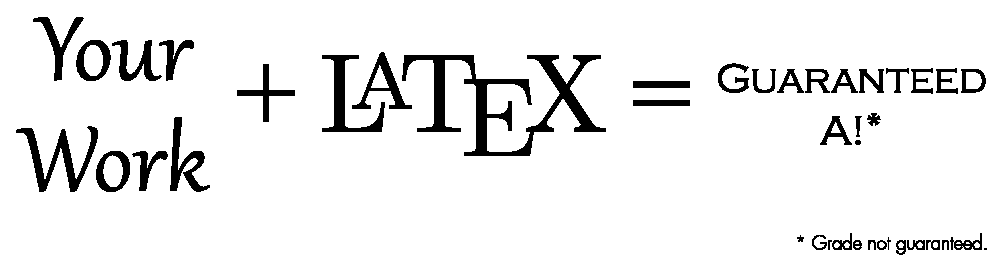
\includegraphics[width=\linewidth]{aplus.eps}
\end{figure*}

To use this document as guide for \LaTeX{}, you will need to refer to
both  the finished PDF file and the .tex file that created it. This means, 
of course, that you will need to have installed a TeX engine on your computer 
(See accompanying README file or just Google it). I have also included the 
.tex code in appendix of this document. Many other (and better) \LaTeX{} 
guides exist.A list of them can be found at http://latex-project.org/guides/.

% NB: LaTeX automatically creates hyperlinks in the digital document
% when http:// is used.

\section{Citations}

When citing, there are a number of different cite commands that allow
for  different sentence structures. \cite{strongrule2012wizards},
\citeA{strongrule2012wizards}, \citeauthor{strongrule2012wizards}, and
\citeyear{strongrule2012wizards} were all created using a different versions of
the {\tt \textbackslash{cite}} command (for above, specifically:
{\tt \textbackslash{cite}}, {\tt \textbackslash{citeA}},{\tt
  \textbackslash{citeauthor}}, and {\tt \textbackslash{citeyear}}). Multiple 
citations can be created by simply including two or more cite keys in the cite
 command separated by a comma: 
\cite{philosophicus1927agenda, strongrule2012wizards}.

% NB: Because certain LaTeX symbols have special meaning in the code
% (& % $ # _ { } ~ ^ \), you have to ``escape" them if you want to
% print them in the text. In cases like those found in the preceding
% paragraph, use the command as shown in the final PDF.

For citations to work, you need an associated .bib file. This is the file 
that holds all the bibliographic information that your sources contain. Many 
PDF managers such as Mendeley will create .bib files for the various working 
folders/libraries you use. Most research databases and Google Scholar will also 
let you export citations in BibTeX format. For citations to populate throughout 
the document properly, your .bib file has to be in the same directory/folder as 
the .tex document or the \LaTeX{} editor you use has to know where to find the 
.bib file (i.e., hard links in the .tex document).

\section{Lists}

You can create a few different types of lists in \LaTeX{}. Three
examples are: enumerate, itemize, description.

\subsection{Enumerate}
\begin{enumerate}[I.] % With the enumerate package, we can change the marker
\item Make a point
\begin{enumerate} % To start a subgroup, just nest another enumerate area
\item Subpoint
\item Subpoint
\end{enumerate}
\item Make another point
\end{enumerate}

\subsection{Itemize}
\begin{itemize}
\item Just
\item some
\item unordered
\item ideas
\end{itemize}

\subsection{Description}
\begin{description}
\item[Put brackets] around the items you want bolded. With enough
  text, you can see that the paragraph is set up with a hanging indent.
\item[Description] is good for defining terms.
\end{description}

\section{Equations}

One of the strengths of \LaTeX{} is its ability to create very nice
equations. As is the case for the entire system, learning the various
equation codes is a pain at first, but worth it in the end.

You can produce inline equations by surrounding the
equation with {\tt \$$\ldots$\$}. An inline equation becomes a bit
squished like so, $\lim_{N \rightarrow \infty} \Pr(\vert \Theta_{N} -
\Theta \vert < \epsilon) = 1$, but inline is good if you only have one
equation within a large body of text. To create full equations that
are numbered, use the \texttt{\textbackslash{begin\{equation\}}} command.

% Begin equation
\begin{equation}
\lim_{N \rightarrow \infty} \Pr(\vert \Theta_{N} - \Theta \vert < \epsilon) = 1
\end{equation}
% End equation

To create an equation without numbering, simply add an asterisk to the
prior command (make sure you have the {\itshape amsmath} package in the
preamble): \texttt{\textbackslash{begin\{equation*\}}}. (Note that
adding an asterisk is the general method for suppressing numbering in
all \LaTeX{} commands that normally add them.) This example equation only 
scratches the surface. There are many more types of equations that \LaTeX{} 
can create. Having a handy symbol guide and a little patience is recommended.


\section{Tables}

\subsection{Everyday Tables}
Tables in \LaTeX{} are the jam. Table \ref{tab:easy} is an easy
one. Notice how Table \ref{tab:easy} is small and without much
text. Had we used more text, \LaTeX{} would have kept it all on one
line and pushed the table outside of the page margins. There are two
ways to have the text wrap and/or set the table to the dimension you
want. The first way is to use the {\itshape tabularx} package. With
{\itshape tabularx} \LaTeX{} can adjust the table to fit whatever
dimensions you set. Table \ref{tab:medium} is an example. If you are a
control freak and absolutely need your table to be a certain size, you
can also set your columns to be specific widths as in Table \ref{tab:mediumer}.

% Easy Table
% h = here
% ! = really
% [!h] = really try to place the thing right here
\begin{table}[!h]
\centering % table align center; otherwise it follows document style
\caption{Easy Table}\label{tab:easy}
% The ``l c r" says that I want three columns that are left aligned,
% center aligned, and  right aligned, respectively. Make sure the
% number of  columns here matches the number you need.
\begin{tabular}{l c r}
\hline % creates a horizontal line
1 & 2 & 3 \\ % Use & to separate columns and \\ to end a line.
\hline
\\ % This gives some space between rows
A & B & C \\
\\
a & b & c \\
\\
$\alpha$ & $\beta$ & $\gamma$ \\
\\
\hline
\end{tabular}
\end{table}

% Medium Table (tabularx)
\begin{table}[!h]
\centering
\caption{Medium Table}\label{tab:medium}
% The X tells LaTeX to set the column width as it sees best; with
% tabularx, you also need to set an overall width in brackets before
% the column brackets. Here, I've told it to be as wide as the length
% a line (i.e. the writable area within the margins).
\begin{tabularx}{\linewidth}{X X X}
\hline
1 & 2 & 3\\
\hline
\\
A & B & C \\
\\
a & b & c \\
\\
$\alpha$ & $\beta$ & $\gamma$ \\
\\
\hline
\end{tabularx}
\end{table}

% Mediumer Table (fixed width column)
\begin{table}[!h]
\centering
\caption{Extra Medium Table}\label{tab:mediumer}
 % The p{} tells the column how wide to be; the >{} before it tells it
 % how to align. You can see that I use some of my homemade commands
 % from above. \RR is much quicker to type than \raggedright\arraybackslash.
\begin{tabular}{>{\RR}p{1in} >{\centering}p{2in} >{\RL}p{1in}}
\hline
1 & 2 & 3\\
\hline
\\
A & B & C \\
\\
a & b & c \\
\\
$\alpha$ & $\beta$ & $\gamma$ \\
\\
\hline
\end{tabular}
\end{table}

\subsection{Cleaner Tables}
Using \texttt{\textbackslash{}hline} when creating tables is a pain,
especially if you want lines that only cover part of the
table. Furthermore, you end up with squished tables. The
{\itshape booktabs} package makes this process easier. See Table
\ref{tab:bettertable} for an example of a slightly more complex, but
more professional-looking table.

% Better Table
\begin{table}[!h]
\centering
\caption{Better Table}\label{tab:bettertable}
\begin{tabular}{>{\RR}p{2in} c c c c}
\toprule
& \multicolumn{2}{l}{Group 1} & \multicolumn{2}{l}{Group 2} \\
\cmidrule(r){2-3}
\cmidrule(r){4-5}
1 & 2 & 3 & 4 & 5\\
\midrule
\\ % This gives some space between rows
A & B & C & D & E\\
\\
a & b & c & d & e\\
\\
$\alpha$ & $\beta$ & $\gamma$ & $\delta$ & $\epsilon$ \\
\\
\bottomrule
\end{tabular}
\end{table}

\subsection{Long Tables}
Sometimes you have a table that is too long and must be spread over
multiple pages. Since the whole point of \LaTeX{} is that it
automatically sets up your document, you need a table that will flow
and break with the page as necessary. The {\itshape longtable} package
allows you to do this. I'm not going to lie, it's a pain to set
up. See Table \ref{tab:long}.

% Long Table
\begin{longtable}{>{\RR}p{2in}>{\centering}p{2in}>{\RL}p{2in}}
\label{tab:long} \\
\caption{Long Table} \\
\toprule % Begin first header
Letter & Number & Greek \\
\midrule
\endfirsthead % End of first header
\multicolumn{2}{l}{\emph{... table \thetable{} continued}} \\ % pb header
\toprule % Repeat header for use after page break (should be the same)
Letter & Number & Greek \\
\midrule
\endhead % all headers finished
\bottomrule % putting in footer before content (way this table works)
\multicolumn{2}{r}{\emph{Continued on next page...}}\\ % pb footer
\endfoot % end of footer
\endlastfoot % since the footer won't change, we can just finish all footers
\\
A & 1 & $\alpha$ \\
\\
B & 2 & $\beta$ \\
\\
C & 3 & $\gamma$ \\
\\
D & 4 & $\delta$ \\
\\
E & 5 & $\epsilon$ \\
\\
F & 6 & $\zeta$ \\
\\
G & 7 & $\eta$ \\
\\
H & 8 & $\theta$ \\
\\
I & 9 & $\iota$ \\
\\
J & 10 & $\kappa$ \\
\\
K & 11 & $\lambda$ \\
\\
L & 12 & $\mu$ \\
\\
M & 13 & $\nu$ \\
\\
N & 14 & $\xi$ \\
\\
O & 15 & $\pi$ \\
\\
P & 16 & $\rho$ \\
\\
Q & 17 & $\sigma$ \\
\\
R & 18 & $\tau$ \\
\\
S & 19 & $\upsilon$ \\
\\
T & 20 & $\phi$ \\
\\
U & 21 & $\chi$ \\
\\
V & 22 & $\psi$ \\
\\
W & 23 & $\omega$ \\
\\
X & 24 &  \\
\\
Y & 25 &  \\
\\
Z & 26 &  \\
\bottomrule
\end{longtable}

\subsection{Tables with External Data}
As you can see from the accompanying .tex file, I've created all the
preceding tables by  hand. While this works for one-off tables with
data that don't change, you want to create tables that will change
automatically if the data coming from a statistical package such as R or
Stata change. The good news is that all you need to do to use an
external table is link to it with the \texttt{\textbackslash{}input}
command in the body of the table. Table \ref{tab:linkeddata} is an
example. Though it looks just like Table \ref{tab:bettertable} in the
formatted PDF, see the .tex file for the difference.

(Of course, I just saved the same data I created before in another
.tex file; to produce the .tex data file automatically with your
favorite statistical software is another matter. My suggestion is to
have the stats software export the data in a .tex format with the
least amount of column, row, and header information possible and use
\LaTeX{} to recreate it: it will look better that way IMNSHO. The
{\itshape estout} package in Stata, with its suite of commands, would be
one way to do this. The {\itshape texreg} library works in R.)

% Better Table (with external file)
\begin{table}[!h]
\centering
\caption{Better Table (with External Data File)}\label{tab:linkeddata}
\begin{tabular}{>{\RR}p{2in} l l l l}
\toprule
& \multicolumn{2}{l}{Group 1} & \multicolumn{2}{l}{Group 2} \\
\cmidrule(r){2-3}
\cmidrule(r){4-5}
1 & 2 & 3 & 4 & 5\\
\midrule
\\ % This gives some space between rows
A & B & C & D & E\\
\\ 
a & b & c & d & e\\
\\
$\alpha$ & $\beta$ & $\gamma$ & $\delta$ & $\epsilon$ \\
\\
\bottomrule
\end{tabular}
\end{table}

\subsection{Sideways Tables}
Other times you need a wide table that is longer than the width of the
page in landscape view. Make sure you have the rotating package called
in the header of the document and simply use the
\texttt{\textbackslash{}sidewaystable} to rotate it. See Table
\ref{tab:sideways} on page \pageref{tab:sideways}.

% Better Table
\begin{sidewaystable} % Use sidewaystable command to rotate table
\centering
\caption{Sideways Table}\label{tab:sideways}
\begin{tabular}{>{\RR}p{3.5in}>{\RR}p{1in}>{\RR}p{1in}>{\RR}p{1in}>{\RR}p{1in}}
\toprule
& \multicolumn{2}{l}{Group 1} & \multicolumn{2}{l}{Group 2} \\
\cmidrule(r){2-3}
\cmidrule(r){4-5}
1 & 2 & 3 & 4 & 5\\
\midrule
\\ % This gives some space between rows
A & B & C & D & E\\
\\
a & b & c & d & e\\
\\
$\alpha$ & $\beta$ & $\gamma$ & $\delta$ & $\epsilon$ \\
\\
\bottomrule
\end{tabular}
\end{sidewaystable}

% Move this part to a new page; sometimes makes things a little
% cleaner, but use sparingly and only at the end...don't fight LaTeX,
% it formats as it does for a reason!
\cleardoublepage

\section{Within Document References}
Another great thing about \LaTeX{} is its ability to create and follow
internal links. When the document is set up correctly, the order of
tables, figures, sections, etc., and the pages they fall on will not
matter for in-text referencing. For example, if you decide to move
Table \ref{tab:easy} to new section, you won't need to relabel with a
different number or change references to it or its page number. When
referencing a table, simply use the \texttt{\textbackslash{}ref}
command with the label you have given the figure (using the
\texttt{\textbackslash{}label} you've given it within the
figure). \LaTeX{} will handle setting up the correct numbers. See the
.tex file for examples throughout.

Similarly, the slick table of contents at the beginning of the
document was created automatically with the
\texttt{\textbackslash{}tableofcontents} command at the beginning of
the document.

\section{Bibliography}
If you don't end up using \LaTeX{} to write papers, you will never
need to worry about a bibliography. If you are slightly mad (and
mostly awesome), then you will use \LaTeX{} for your all your 
finished papers.

To create a bibliography, simply include
\texttt{\textbackslash{}bibliography\{{\itshape nameofyourbibfile\}}} at
the end of your .tex file. You probably also want to include
\texttt{\textbackslash{}bibliographystyle} so that you can control how
the bibliography looks. To create this document, I've used the
\texttt{apacite.sty} (.sty means style$\ldots$I assume) within the
\texttt{\textbackslash{}bibliographystyle} brackets. I've also
included the \texttt{\textbackslash{}urlstyle\{same\}} command. This
prevents the url links in the bibliography entries, should I have any,
from formatting in monospace font. To use the \texttt{apacite.sty},
note that I've include the \texttt{apacite} package in the header of
my .tex file.


%% END BODY %%%%%%%%%%%%%%%%%%%%%%%%%%%%%%%%%%%%%%%%%%%%%%%%%%%%%%%%%%%%%%%%
%% BEGIN BIBLIOGRAPHY %%%%%%%%%%%%%%%%%%%%%%%%%%%%%%%%%%%%%%%%%%%%%%%%%%%%%%

\cleardoublepage
\bibliographystyle{apacite}
\urlstyle{same}
\bibliography{LatexExample}

%% END BIBLIOGRAPHY %%%%%%%%%%%%%%%%%%%%%%%%%%%%%%%%%%%%%%%%%%%%%%%%%%%%%%%%
\end{verbatim}

\section{Latex External Table Code}
\footnotesize
\begin{verbatim}
A & B & C & D & E\\
\\ 
a & b & c & d & e\\
\\
$\alpha$ & $\beta$ & $\gamma$ & $\delta$ & $\epsilon$ \\
\end{verbatim}

\section{External .bib File Example}
\footnotesize
\begin{verbatim}
@article{philosophicus1927agenda,
        Author = {Philosophicus, Publius},
        Journal = {The National Eschew},
        Number = 7,
        Pages = {23--40},
        Title = {The Liberal {LaTeX} Agenda},
        Volume = 5,
        Year = 1927
}

@book{strongrule2012wizards,
        Author = {Strongrule, Lucky},
        Publisher = {Muggle Press},
        Title = {Wizards Don't Walk: The case against slytherin' and all
                 forms of bipedalism},
        Year = 1992
}

@book{watterson1992indesp,
        Author = {Watterson, Bill},
        Publisher = {Andrews McMeel Publishing},
        Title = {{The Indispensable Calvin and Hobbes: 
                A Calvin and Hobbes Treasury}},
        Year = {1992}
}
\end{verbatim}


\end{document}
